\documentclass[tikz,border=2pt]{standalone}
\usepackage{tkz-euclide}

\begin{document}
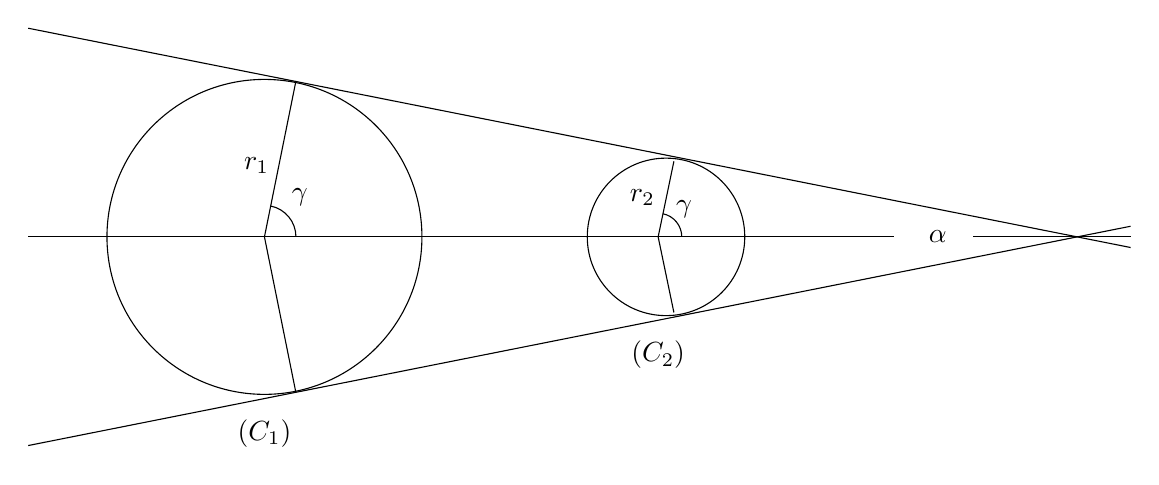
\begin{tikzpicture}

  \tkzDefPoints{0/0/A, 0.4/1.98/B, 5/0/C, 5.2/0.96/D}

  \draw (0,0) circle (2);
  \draw (5.1,0) circle (1);

  % Tangent lines
  \draw (-3,-2.65) -- (11,0.135);
  \draw (-3,2.65) -- (11,-0.135);

  \draw (0, 0) -- (0.4, 1.98);
  \draw (0, 0) -- (0.4, -1.98);

  \draw (5, 0) -- (5.2, 0.96);
  \draw (5, 0) -- (5.2, -0.96);

  \draw (-3, 0) -- (8, 0);
  \draw (9,0) -- (11,0);

  \tkzMarkAngle[size=0.4](C,A,B)
  \tkzMarkAngle[size=0.3, xshift=5cm, yshift=0cm](C,A,B)

  \node at (0,-2.5) {$(C_1)$};
  \node at (5,-1.5) {$(C_2)$};
  \node at (-0.1, 0.91) {$r_{1}$};
  \node at (0.45, 0.5) {$\gamma$};
  \node at (4.8, 0.5) {$r_{2}$};
  \node at (5.33, 0.35) {$\gamma$};
  \node at (8.55,0) {$\alpha$};

\end{tikzpicture}
\end{document}
